\subsection{Entfernen der Login und SignUp Klasse}
Während der Implementierung der UserAdministration, ist schnell aufgefallen, dass sowohl Login- als auch SignUp keine benötigten Klassen sind.
Stattdessen ist die Logik von Login und SignUp nun in der UserController Klasse beinhaltet.

\begin{figure}[h]
            \label{UserAdministration}
            \centerline{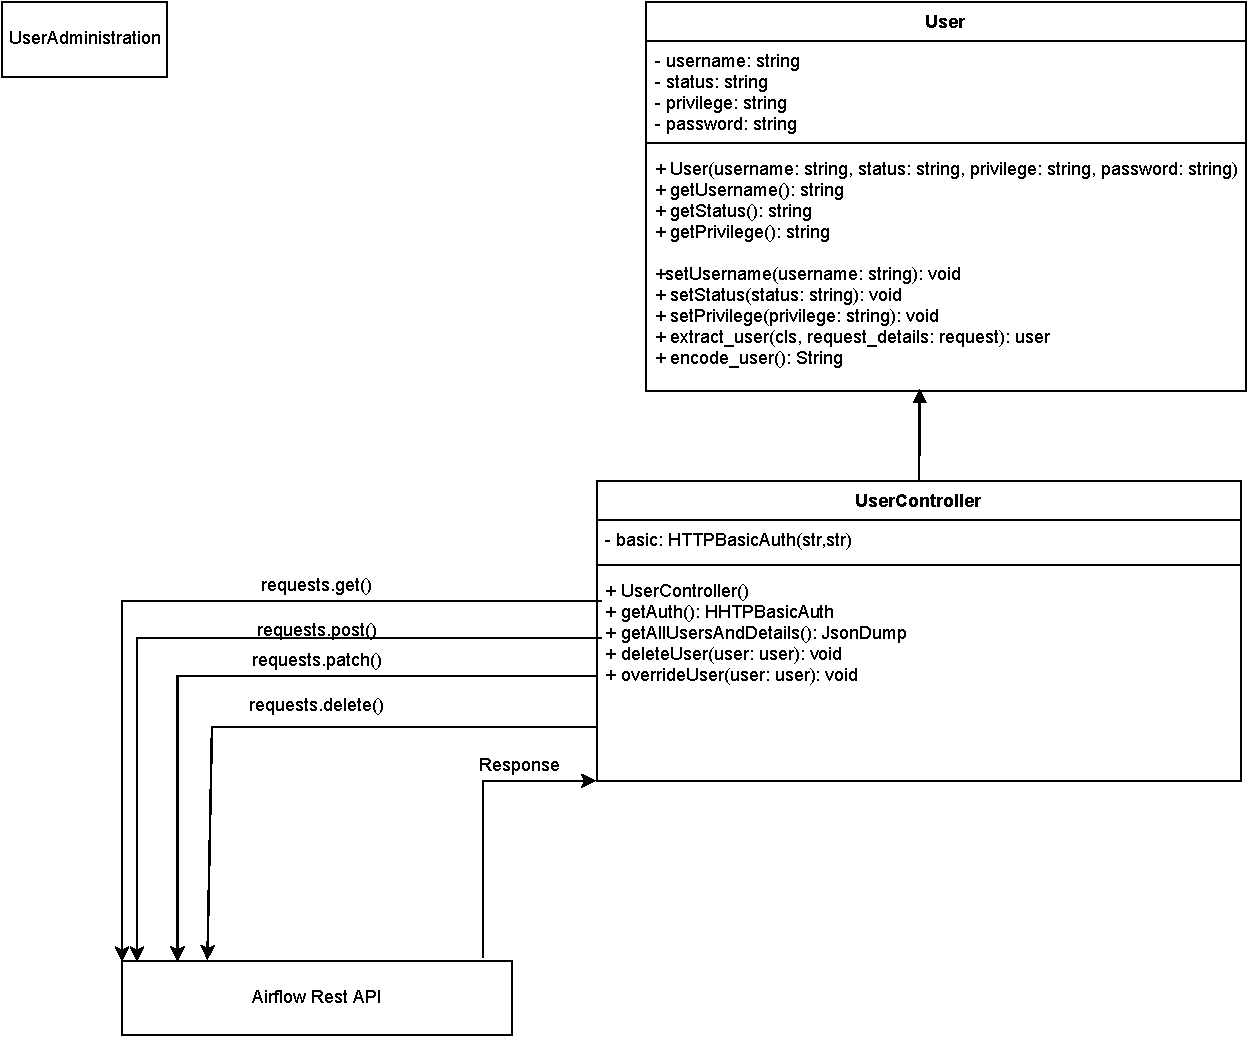
\includegraphics[scale=0.7]{res/UserAdministration.pdf}}
            \caption{Die überarbeitete Version der UserAdministration}
\end{figure}

In dem Diagramm wurden die 2 Redundanten Klassen entfernt und neue Methoden hinzugefügt. Des Weiteren ist die Schnittstelle zu Airflow nun genauer definiert worden.